\documentclass[aspectratio=169]{beamer}

\usetheme{Boadilla}
\usefonttheme{professionalfonts}
\setbeamertemplate{navigation symbols}{}
\setbeamertemplate{itemize items}[circle]
\setbeamertemplate{enumerate items}[default]
\setbeamertemplate{headline}{}

\usepackage[utf8]{inputenc}
\usepackage[T1]{fontenc}
\usepackage{lmodern}
\usepackage{amsmath}
\usepackage{booktabs}
\usepackage{tabularx}
\usepackage{array}
\usepackage{hyperref}
\usepackage[strings]{underscore}
\usepackage{listings}
\usepackage{tikz}
\usetikzlibrary{arrows.meta,positioning,fit,calc,shapes.geometric}
\usepackage{xcolor}

\definecolor{courseblue}{HTML}{12355B}
\definecolor{coursegold}{HTML}{C98A2E}
\definecolor{courseice}{HTML}{EEF3F8}
\definecolor{coursegreen}{HTML}{2F6B4F}
\definecolor{coursegray}{HTML}{4B5563}
\definecolor{codebg}{HTML}{F7F9FC}
\definecolor{codecomment}{HTML}{5E6C84}
\definecolor{codestring}{HTML}{0B6E4F}

\setbeamercolor{palette primary}{bg=courseblue,fg=white}
\setbeamercolor{palette secondary}{bg=coursegold,fg=white}
\setbeamercolor{palette tertiary}{bg=courseblue,fg=white}
\setbeamercolor{palette quaternary}{bg=coursegold,fg=white}
\setbeamercolor{structure}{fg=courseblue}
\setbeamercolor{frametitle}{bg=courseice,fg=courseblue}
\setbeamercolor{title}{fg=courseblue}
\setbeamercolor{block title}{bg=courseblue,fg=white}
\setbeamercolor{block body}{bg=courseice,fg=black}
\setbeamercolor{normal text}{fg=black,bg=white}
\setbeamercolor{alerted text}{fg=coursegold}

\setbeamerfont{footline}{size=\scriptsize}

\setbeamertemplate{footline}{
  \leavevmode
  \hbox{
    \begin{beamercolorbox}[wd=.33\paperwidth,ht=2.8ex,dp=1.2ex,leftskip=0.8em]{palette primary}%
      University of Trieste
    \end{beamercolorbox}%
    \begin{beamercolorbox}[wd=.49\paperwidth,ht=2.8ex,dp=1.2ex,center]{palette tertiary}%
      \coursename{} \textbar{} \coursecode
    \end{beamercolorbox}%
    \begin{beamercolorbox}[wd=.18\paperwidth,ht=2.8ex,dp=1.2ex,rightskip=0.8em plus1fil]{palette secondary}%
      \insertframenumber{} / \inserttotalframenumber
    \end{beamercolorbox}%
  }
}

\hypersetup{
  colorlinks=true,
  linkcolor=courseblue,
  urlcolor=coursegreen
}

\lstdefinestyle{coursepython}{
  language=Python,
  basicstyle=\ttfamily\footnotesize,
  keywordstyle=\color{courseblue}\bfseries,
  commentstyle=\color{codecomment}\itshape,
  stringstyle=\color{codestring},
  showstringspaces=false,
  columns=fullflexible,
  keepspaces=true,
  frame=single,
  framerule=0.6pt,
  rulecolor=\color{courseblue},
  backgroundcolor=\color{codebg},
  xleftmargin=0.4em,
  xrightmargin=0.4em,
  aboveskip=0.4em,
  belowskip=0.2em
}

\newcommand{\coursename}{Data-driven Systems Engineering}
\newcommand{\coursecode}{440MI / 305SM}
\newcommand{\coursefooter}{}

\newcommand{\learninggoals}[1]{
  \begin{block}{Learning goals}
  #1
  \end{block}
}

\newcommand{\repoactivity}[1]{
  \begin{block}{Repo activity}
  #1
  \end{block}
}

\newcommand{\readinglist}[1]{
  \begin{block}{Papers and materials}
  {\footnotesize #1}
  \end{block}
}

\newcommand{\coursecontextframe}[5]{
  \begin{frame}{Course Map and Running Cases}
  \centering
  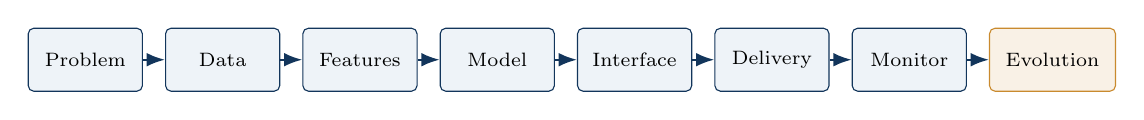
\begin{tikzpicture}[node distance=0.28cm]
  \node[flowbox, minimum width=1.45cm, minimum height=0.8cm] (problem) {\scriptsize Problem};
  \node[flowbox, minimum width=1.45cm, minimum height=0.8cm, right=of problem] (data) {\scriptsize Data};
  \node[flowbox, minimum width=1.45cm, minimum height=0.8cm, right=of data] (features) {\scriptsize Features};
  \node[flowbox, minimum width=1.45cm, minimum height=0.8cm, right=of features] (model) {\scriptsize Model};
  \node[flowbox, minimum width=1.45cm, minimum height=0.8cm, right=of model] (interface) {\scriptsize Interface};
  \node[flowbox, minimum width=1.45cm, minimum height=0.8cm, right=of interface] (delivery) {\scriptsize Delivery};
  \node[flowbox, minimum width=1.45cm, minimum height=0.8cm, right=of delivery] (monitor) {\scriptsize Monitor};
  \node[accentbox, minimum width=1.6cm, minimum height=0.8cm, right=of monitor] (evolution) {\scriptsize Evolution};
  \foreach \a/\b in {problem/data,data/features,features/model,model/interface,interface/delivery,delivery/monitor,monitor/evolution} {
    \draw[arrow] (\a) -- (\b);
  }
  \end{tikzpicture}

  \vspace{0.5em}
  \begin{block}{Today in the course}
  \textbf{Focus:} #1

  \textbf{Bridge:} #2
  \end{block}

  \begin{columns}[T]
  \column{0.48\textwidth}
  \begin{block}{Fraud case}
  {\footnotesize #3}
  \end{block}
  \column{0.48\textwidth}
  \begin{block}{Pasteurization case}
  {\footnotesize #4}
  \end{block}
  \end{columns}

  \vspace{0.3em}
  {\footnotesize \textbf{Course thread:} #5}
  \coursefooter
  \end{frame}
}

\newcommand{\classclosingframe}[4]{
  \begin{frame}{From This Class to the Next}
  \begin{block}{What stays with us}
  #1
  \end{block}

  \begin{columns}[T]
  \column{0.48\textwidth}
  \begin{block}{Project use}
  {\footnotesize #2}
  \end{block}
  \column{0.48\textwidth}
  \begin{block}{Next connection}
  {\footnotesize #3}
  \end{block}
  \end{columns}

  \vspace{0.3em}
  {\footnotesize \textbf{Course thread:} #4}
  \coursefooter
  \end{frame}
}

\tikzset{
  flowbox/.style={
    rounded corners=3pt,
    draw=courseblue,
    fill=courseice,
    very thick,
    minimum width=2.2cm,
    minimum height=0.9cm,
    align=center,
    font=\small
  },
  accentbox/.style={
    rounded corners=3pt,
    draw=coursegold,
    fill=coursegold!15,
    very thick,
    minimum width=2.2cm,
    minimum height=0.9cm,
    align=center,
    font=\small
  },
  arrow/.style={
    -{Latex[length=2.5mm,width=2mm]},
    thick,
    draw=courseblue
  }
}


% Keep the diagram dimensions used by this deck.
\tikzset{flowbox/.style={draw=courseblue,fill=courseice,rounded corners=2pt,align=center},
accentbox/.style={draw=coursegold,fill=coursegold!12,rounded corners=2pt,align=center},
arrow/.style={-Latex,thick,draw=courseblue}}

% Stage navigation: the active item uses the course accent colour.
\newcommand{\pipelinefocus}[1]{%
\begin{center}
\begin{tikzpicture}[node distance=0.22cm,
  stage/.style={draw=courseblue,fill=courseice,rounded corners=2pt,
    minimum width=1.95cm,minimum height=0.55cm,inner sep=3pt,font=\small,align=center},
  active/.style={draw=coursegold,fill=coursegold!22,line width=1.2pt,font=\small\bfseries}]
\foreach \label [count=\i] in {Raw data,Clean,Construct,Represent,Select,Model}{
  \ifnum\i=1
    \node[stage] (stage\i) at (0,0) {\label};
  \else
    \pgfmathtruncatemacro{\previous}{\i-1}
    \node[stage,right=of stage\previous] (stage\i) {\label};
    \draw[arrow] (stage\previous) -- (stage\i);
  \fi
  \ifnum\i=#1
    \node[stage,active] at (stage\i.center) {\label};
  \fi
}
\end{tikzpicture}
\end{center}
\vspace{-0.3em}
}

% Pipeline with a parallel track: a bar spanning every stage.
\newcommand{\pipelineparallel}[1]{%
\begin{center}
\begin{tikzpicture}[node distance=0.22cm,
  stage/.style={draw=courseblue,fill=courseice,rounded corners=2pt,
    minimum width=1.95cm,minimum height=0.55cm,inner sep=3pt,font=\small,align=center}]
\foreach \label [count=\i] in {Raw data,Clean,Construct,Represent,Select,Model}{
  \ifnum\i=1
    \node[stage] (stage\i) at (0,0) {\label};
  \else
    \pgfmathtruncatemacro{\previous}{\i-1}
    \node[stage,right=of stage\previous] (stage\i) {\label};
    \draw[arrow] (stage\previous) -- (stage\i);
  \fi
}
\path (stage1.south west) ++(0,-0.3cm) coordinate (barnw);
\path (stage6.south east) ++(0,-0.85cm) coordinate (barse);
\draw[accentbox] (barnw) rectangle (barse);
\node[font=\small\bfseries] at ($(barnw)!0.5!(barse)$) {#1};
\foreach \i in {1,...,6}{\draw[coursegold,dashed] (stage\i.south) -- (stage\i.south |- barnw);}
\end{tikzpicture}
\end{center}
\vspace{-0.3em}
}

% Preserves references to original illustrations without preventing compilation
% when only the .tex file is available.
\newcommand{\optionalfigure}[2]{%
\IfFileExists{#1}{\includegraphics[#2]{#1}}{%
\fcolorbox{courseblue}{courseice}{\parbox[c][3.0cm][c]{0.82\linewidth}{\centering\footnotesize Original figure not bundled\\[0.4em]\texttt{\detokenize{#1}}\\[0.4em]Copy the original images/ folder here.}}}}


\title{Class 16: Feature Engineering --- From Raw Data to Validated Features}
\author{\coursename}
\date{}

\begin{document}

\frame{\titlepage \coursefooter}

\begin{frame}{Agenda}
\begin{itemize}
\item Data curation and cleaning: missing values, duplicates, invalid values, outliers.
\item Feature construction and representation: domain knowledge, encoding, scaling, PCA.
\item Feature selection: filter and wrapper methods.
\item Leakage checks and the Titanic case: baseline, ablation, reproducible pipeline.
\end{itemize}
\coursefooter
\end{frame}
\begin{frame}{Encoding as part of feature engineering}
\begin{itemize}
\item Encoding is one component of feature engineering, alongside cleaning, construction, scaling, and selection.
\item Data cleaning addresses missing values, duplicates, and inconsistent types; encoding determines how categories are represented numerically.
\item Not every available variable should become a feature: some are redundant, some carry only noise, and some induce leakage.
\item Informative features are frequently absent from the raw data and must be constructed from domain knowledge.
\end{itemize}
\coursefooter
\end{frame}
\begin{frame}{Feature engineering in the modeling workflow}
\centering
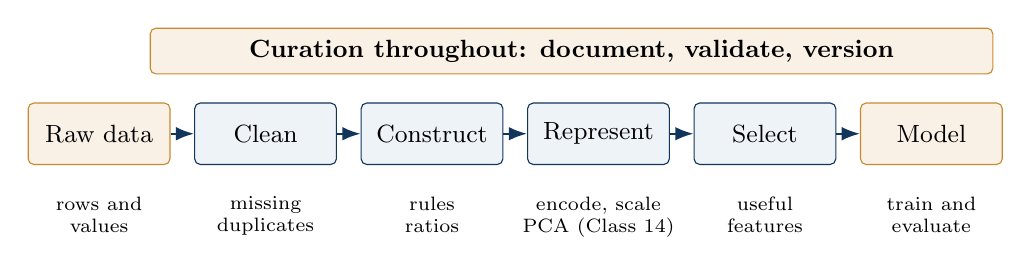
\begin{tikzpicture}[node distance=0.3cm]
\node[accentbox, minimum width=1.8cm, minimum height=0.78cm, font=\small] (raw) {Raw data};
\node[flowbox, minimum width=1.8cm, minimum height=0.78cm, font=\small, right=of raw] (clean) {Clean};
\node[flowbox, minimum width=1.8cm, minimum height=0.78cm, font=\small, right=of clean] (construct) {Construct};
\node[flowbox, minimum width=1.8cm, minimum height=0.78cm, font=\small, right=of construct] (encode) {Represent};
\node[flowbox, minimum width=1.8cm, minimum height=0.78cm, font=\small, right=of encode] (select) {Select};
\node[accentbox, minimum width=1.8cm, minimum height=0.78cm, font=\small, right=of select] (model) {Model};
\draw[arrow] (raw) -- (clean);
\draw[arrow] (clean) -- (construct);
\draw[arrow] (construct) -- (encode);
\draw[arrow] (encode) -- (select);
\draw[arrow] (select) -- (model);
\node[below=0.28cm of raw, font=\scriptsize, align=center] {rows and\\values};
\node[below=0.28cm of clean, font=\scriptsize, align=center] {missing\\duplicates};
\node[below=0.28cm of construct, font=\scriptsize, align=center] {rules\\ratios};
\node[below=0.28cm of encode, font=\scriptsize, align=center] {encode, scale\\PCA (Class 14)};
\node[below=0.28cm of select, font=\scriptsize, align=center] {useful\\features};
\node[below=0.28cm of model, font=\scriptsize, align=center] {train and\\evaluate};
\node[accentbox, minimum width=10.7cm, minimum height=0.58cm, font=\small\bfseries] at (6.0,1.05) {Curation throughout: document, validate, version};
\end{tikzpicture}

\vspace{0.25em}
\begin{block}{Feature construction and transformation}
\centering\small
Construction creates candidate features (e.g., ratios or rolling means). It is one kind of feature transformation; encoding and scaling also transform features, while selection chooses which candidates to keep.
\end{block}
\vspace{-0.25em}
{\scriptsize The workflow is iterative: reject leaking or unavailable features early; construction and selection may be revisited. PCA constructs components rather than selecting original columns.}
\coursefooter
\end{frame}
\begin{frame}{Raw data: the starting point}
\pipelinefocus{1}
\begin{columns}[T]
\column{0.52\textwidth}
\begin{block}{What is raw data?}\small
Data exactly as collected or exported from its source, before cleaning, construction, or encoding. Each row is an observation; each column is an attribute.
\end{block}
\begin{itemize}\small
\item \textbf{Types:} numeric, categorical, text, timestamp, stream.
\item \textbf{Granularity:} what one row represents.
\item \textbf{Provenance:} source, date, version.
\end{itemize}
\column{0.44\textwidth}
\begin{block}{What to expect in raw data}\small
\begin{itemize}
\item Missing and duplicated values
\item Inconsistent types or units
\item Outliers and invalid entries
\item Identifiers and leaking columns
\end{itemize}
\end{block}
\end{columns}
\vspace{-0.2em}
\begin{alertblock}{Good practice}\small
Keep an untouched copy; apply every change in code.
\end{alertblock}
\coursefooter
\end{frame}
\begin{frame}{Running case: Titanic survival prediction}
\begin{block}{Engineering question}
Can we predict whether a passenger survives, using only information available at the intended prediction moment?
\end{block}
\begin{columns}[T]
\column{0.52\textwidth}
\begin{itemize}\small
\item \textbf{Target:} \texttt{survived} (binary), $n=891$ passengers.
\item \textbf{Source:} classic Kaggle training set: 12 columns, including the target and passenger identifier.
\item \textbf{Candidates:} 10 original passenger attributes; derived features must have explicit definitions.
\end{itemize}
\column{0.46\textwidth}
\begin{block}{Evidence we will reveal}\small
Raw $\rightarrow$ Curate $\rightarrow$ Clean $\rightarrow$ Construct $\rightarrow$ Represent $\rightarrow$ Select $\rightarrow$ Validate.
\end{block}
\end{columns}
\vspace{0.3em}
\textbf{Class discussion:} Is a variable useful just because it is predictive?
\coursefooter
\end{frame}

\begin{frame}{Data curation}
\pipelineparallel{Data curation: document, validate, version}
\begin{itemize}
\item Curation makes a dataset understandable and reusable beyond its original authors.
\item A data dictionary records the meaning, unit, and valid range of every column.
\item Capture provenance and lineage: source, extraction/query, timestamp, version, and feature definitions; an extraction date alone does not guarantee reproducibility.
\item Validation rules (schema and range checks) detect upstream problems before they reach the modeling stage.
\end{itemize}
\begin{block}{Repository example}
For Titanic, record a feature contract: definition, type, allowed values, missingness policy, source, prediction-time availability, and version. The fraud-case specification in \texttt{documents/FraudDetectionAsaService.pdf} illustrates similar documentation.
\end{block}
\coursefooter
\end{frame}
\begin{frame}{Titanic / 1: curate the feature contract}
\small
\begin{tabularx}{\textwidth}{>{\ttfamily}l l X X}
\normalfont\bfseries Field & \bfseries Type & \bfseries Meaning / validation & \bfseries Prediction-time audit \\
\toprule
survived & binary & Target; 0 or 1 & Never an input \\
sex & nominal & Passenger category & Check available \\
age & numeric & Age in years; missing possible & Check available \\
sibsp & count & Siblings/spouses aboard; $\ge 0$ & Check available \\
parch & count & Parents/children aboard; $\ge 0$ & Check available \\
embarked & nominal & Embarkation port; some missing & Check available \\
passengerid & identifier & Unique passenger key & Exclude from baseline inputs \\
\bottomrule
\end{tabularx}
\vspace{0.5em}
\begin{block}{What should be versioned?}
\small Dataset snapshot / extraction, column schema, validation rules, cleaning and construction code, split definition, and fitted preprocessing artifacts.
\end{block}
\textbf{Question:} Which fields would you reject \emph{before} looking at feature scores?
\coursefooter
\end{frame}
\begin{frame}{Data cleaning: scope and quality dimensions}
\pipelinefocus{2}
\centering
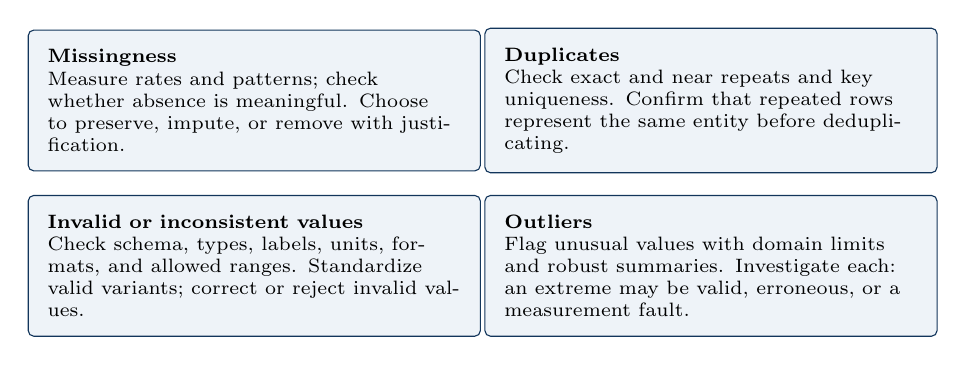
\begin{tikzpicture}
\node[flowbox, text width=5.25cm, minimum height=1.45cm, align=left, inner sep=7pt, font=\scriptsize] at (-2.9,0) {\textbf{Missingness}\\Measure rates and patterns; check whether absence is meaningful. Choose to preserve, impute, or remove with justification.};
\node[flowbox, text width=5.25cm, minimum height=1.45cm, align=left, inner sep=7pt, font=\scriptsize] at (2.9,0) {\textbf{Duplicates}\\Check exact and near repeats and key uniqueness. Confirm that repeated rows represent the same entity before deduplicating.};
\node[flowbox, text width=5.25cm, minimum height=1.45cm, align=left, inner sep=7pt, font=\scriptsize] at (-2.9,-2.1) {\textbf{Invalid or inconsistent values}\\Check schema, types, labels, units, formats, and allowed ranges. Standardize valid variants; correct or reject invalid values.};
\node[flowbox, text width=5.25cm, minimum height=1.45cm, align=left, inner sep=7pt, font=\scriptsize] at (2.9,-2.1) {\textbf{Outliers}\\Flag unusual values with domain limits and robust summaries. Investigate each: an extreme may be valid, erroneous, or a measurement fault.};
\end{tikzpicture}

\vspace{0.2em}
{\footnotesize \textbf{Cleaning is a documented decision, not automatic deletion.} For each issue, record the evidence found, the action taken (keep, correct, impute, or remove), and why that action is justified.}
\coursefooter
\end{frame}
\begin{frame}{Data cleaning: common techniques}
\begingroup\scriptsize
\renewcommand{\arraystretch}{1.1}
\begin{tabularx}{\textwidth}{>{\bfseries}p{2.9cm} >{\raggedright\arraybackslash}X >{\raggedright\arraybackslash}X}
\toprule
Issue & Detect & Treat \\
\midrule
Missing values & Missingness rates and matrix plots; Little's MCAR test & Mean/median/mode imputation; $k$-NN imputation; iterative imputation (MICE); missing-value indicator \\
\addlinespace[0.15em]
Duplicates & Key-uniqueness checks; hashing for exact matches; string similarity (Levenshtein, Jaro--Winkler) for near matches & Record linkage with blocking; MinHash/LSH at scale; keep-first or merge rule \\
\addlinespace[0.15em]
Invalid or inconsistent & Schema and type validation (e.g., pandera, Great Expectations); regular expressions; range and unit checks & Type coercion; category mapping to canonical labels; unit conversion; reject or flag \\
\addlinespace[0.15em]
Outliers & Tukey IQR fences; $z$-score and robust $z$-score (MAD); Isolation Forest; Local Outlier Factor & Winsorizing (capping); log or Box--Cox transform; robust scalers; remove only if erroneous \\
\bottomrule
\end{tabularx}
\par\endgroup
\vspace{0.1em}
\begin{block}{Record and validate}
Document the checks and decisions. Fit imputation within each training fold and apply it unchanged to held-out and production data.
\end{block}
\coursefooter
\end{frame}
\begin{frame}{Titanic / 2: cleaning decisions per column}
\small
\begin{tabularx}{\textwidth}{l l X}
\toprule
Original column & Candidate policy & Assessment / rationale \\
\midrule
\texttt{cabin} & Preserve missingness & Often absent; derive a known/unknown indicator or a deck category with an explicit Unknown level. \\
\texttt{age} & Median imputation & Inspect missingness and distributions; fit the median within each training fold. \\
\texttt{embarked} & Mode or Unknown & Inspect missing entries; fit any mode using the training fold. \\
\texttt{fare} & Validate / impute & Check range, extremes, and missingness in each supplied file. \\
\texttt{passengerid} & Validate uniqueness & Audit repeated identifiers; equal passenger attributes alone do not establish duplicate records. \\
\bottomrule
\end{tabularx}
\coursefooter
\end{frame}
\begin{frame}{Feature construction from domain knowledge}
\pipelinefocus{3}
\begin{block}{What is feature construction?}
Deriving new variables from existing ones, guided by knowledge of the problem, so that a useful pattern becomes easier for the model to use.
\end{block}
\vspace{0.4em}
\textbf{Main methods}
\begin{columns}[T]
\column{0.46\textwidth}
\begin{itemize}
\item Arithmetic combinations
\item Aggregations
\item Binning
\item Indicators and rules
\end{itemize}
\column{0.46\textwidth}
\begin{itemize}
\item Date and time parts
\item Text extraction
\item Interactions
\item Rolling windows
\end{itemize}
\end{columns}
\coursefooter
\end{frame}
\begin{frame}{Streams and sensors: rolling mean and window size}
\begin{columns}[T]
\column{0.62\textwidth}
\centering
\optionalfigure{images/class16_rolling_mean_windows.pdf}{width=\linewidth,height=0.5\textheight,keepaspectratio}

{\tiny One batch generated by \texttt{pasteurization/synth\_sensors.py}.\par}
\vspace{0.3em}
\footnotesize Example with $w=3$:\\[0.2em]
\begin{tabular}{l|ccccc}
$t$ & 1 & 2 & 3 & 4 & 5 \\
\hline
$x_t$ & 10 & 12 & 14 & 20 & 18 \\
$\bar{x}_t$ & -- & -- & 12 & 15.3 & 17.3 \\
\end{tabular}\\[0.2em]
{\scriptsize $\bar{x}_4 = (12+14+20)/3$; the first $w-1$ values are undefined.}
\column{0.36\textwidth}
\footnotesize
\textbf{Rolling mean} of the temperature $T_t$:
\[\bar{T}_t = \frac{1}{w}\sum_{i=0}^{w-1} T_{t-i}\]
\begin{itemize}
\item Small $w$ ($5$): follows the signal closely, little smoothing.
\item Medium $w$ ($15$): removes noise, with a visible delay.
\item Large $w$ ($45$): very smooth, but lags by about $w/2$ samples and flattens the Hold plateau.
\end{itemize}
Choose $w$ to trade noise reduction against delay.
\end{columns}
\coursefooter
\end{frame}
\begin{frame}{Streams and sensors: rate of change}
\begin{columns}[T]
\column{0.62\textwidth}
\centering
\optionalfigure{images/class16_rate_of_change.pdf}{width=\linewidth,height=0.5\textheight,keepaspectratio}

{\tiny One batch generated by \texttt{pasteurization/synth\_sensors.py}.\par}
\vspace{0.3em}
\footnotesize Example with $\Delta t = 1$ s:\\[0.2em]
\begin{tabular}{l|cccccc}
$t$ & 1 & 2 & 3 & 4 & 5 & 6 \\
\hline
state & Idle & Idle & HeatUp & HeatUp & HeatUp & Hold \\
$T_t$ & 20 & 20 & 22 & 25 & 28 & 28 \\
$\dot{T}_t$ & -- & 0 & 2 & 3 & 3 & 0 \\
\end{tabular}
\column{0.36\textwidth}
\footnotesize
\textbf{Rate of change:}
\[\dot{T}_t = \frac{T_t - T_{t-1}}{\Delta t}\]
\begin{itemize}
\item Positive in HeatUp, negative in Cool, near zero elsewhere.
\item The raw value $T_t$ cannot separate these regimes: $28$ °C may be heating or cooling.
\item The first sample is undefined: it has no predecessor.
\end{itemize}
\end{columns}
\coursefooter
\end{frame}
\begin{frame}{Streams and sensors: time in phase}
\begin{columns}[T]
\column{0.62\textwidth}
\centering
\optionalfigure{images/class16_time_in_phase.pdf}{width=\linewidth,height=0.5\textheight,keepaspectratio}

{\tiny One batch generated by \texttt{pasteurization/synth\_sensors.py}.\par}
\vspace{0.3em}
\footnotesize Example with $\Delta t = 1$ s:\\[0.2em]
\begin{tabular}{l|cccccc}
$t$ & 1 & 2 & 3 & 4 & 5 & 6 \\
\hline
state & Idle & Idle & HeatUp & HeatUp & HeatUp & Hold \\
time in phase [s] & 0 & 1 & 0 & 1 & 2 & 0 \\
\end{tabular}
\column{0.36\textwidth}
\footnotesize
\textbf{Time in phase:} seconds since the last change of state.
\begin{itemize}
\item The counter resets to $0$ whenever the state changes.
\item It distinguishes a slow heating from a normal one: the same temperature after $10$ s or $40$ s in HeatUp means different things.
\item It uses only past observations, so it can be computed online, one sample at a time.
\item The state label is categorical: it can be encoded as in Class 14 (e.g., one-hot) and used beside this feature.
\end{itemize}
\end{columns}
\coursefooter
\end{frame}
\begin{frame}{Represent candidates before selection}
\pipelinefocus{4}
\begin{itemize}
\item Selection methods need features in a representation they can use: encode categorical variables and scale numeric ones when the method is scale-sensitive.
\item One-hot, ordinal, target, and cyclic encodings offer different representations; the choice depends on the variable and the model.
\item PCA transforms the feature space into components. It constructs a new representation rather than selecting original columns.
\item Fit imputers, scalers, PCA, target-dependent selectors, and other learned transformations using training folds only; use out-of-fold target encoding.
\end{itemize}
\coursefooter
\end{frame}
\begin{frame}{Feature selection: filter and wrapper}
\pipelinefocus{5}
\begingroup\small
Given $d$ candidate features, selection seeks a subset $S \subseteq \{1, \dots, d\}$ that maximizes a criterion $J(S)$. The two families differ in how $J$ is defined.
\par\endgroup
\vspace{0.5em}
\begin{tabularx}{\textwidth}{>{\bfseries}l X}
Filter & $J$ is a model-independent statistic computed for each feature, e.g.\ correlation, mutual information, or the $\chi^2$ statistic. \\
\addlinespace[0.3em]
Wrapper & $J(S)$ is the validation performance of a model trained on $S$; subsets are explored by a search strategy (e.g.\ forward or backward selection). \\
\bottomrule
\end{tabularx}
\coursefooter
\end{frame}
\begin{frame}{Titanic / 6: engineering changes feature dependencies}
\begin{columns}[T]
\column{0.55\textwidth}
\centering
\optionalfigure{images/class16_titanic_correlation.pdf}{width=\linewidth}
\column{0.43\textwidth}
\begin{itemize}\footnotesize
\item Pearson correlations after cleaning (\texttt{age} imputed with the median).
\item \texttt{family\_size} is strongly correlated with its components \texttt{sibsp} ($0.89$) and \texttt{parch} ($0.78$): keeping all three adds collinearity.
\item \texttt{is\_alone} has a larger linear association with \texttt{survived} ($-0.20$) than \texttt{family\_size} ($0.02$).
\item Pearson measures only linear dependence; a near-zero value does not make a feature uninformative.
\item \textbf{Spearman} is Pearson on ranks: it captures monotonic association and resists outliers. Prefer it for skewed, ordinal, or curved data; use Pearson for roughly linear data.
\end{itemize}
\end{columns}
\coursefooter
\end{frame}
\begin{frame}{Modeling: what it is and main types}
\pipelinefocus{6}
\begin{block}{What is a model?}\small
A function $f_{\theta}$ that maps features to a prediction, $\hat{y} = f_{\theta}(\mathbf{x})$, with parameters $\theta$ estimated from data. Training is the subject of Class 18; experiment tracking and evaluation are the subject of Class 19.
\end{block}
\begin{columns}[T]
\column{0.49\textwidth}
\textbf{By learning paradigm}
\begin{itemize}\footnotesize
\item \textbf{Supervised:} learns from labeled pairs $(\mathbf{x}_i, y_i)$; classification or regression. Titanic: predict \texttt{survived}.
\item \textbf{Unsupervised:} no target; finds structure, e.g.\ clustering or PCA (Class 14).
\item \textbf{Self-supervised:} the target is built from the data itself, e.g.\ word2vec (Class 14).
\item \textbf{Reinforcement:} learns from rewards obtained by interacting with an environment.
\end{itemize}
\column{0.49\textwidth}
\textbf{By model family}
\begin{itemize}\footnotesize
\item \textbf{Linear:} linear and logistic regression; interpretable.
\item \textbf{Tree-based:} decision trees, random forests, gradient boosting; capture non-linearity.
\item \textbf{Instance-based:} $k$-nearest neighbours.
\item \textbf{Neural networks:} multilayer perceptrons, CNNs, RNNs; see Class 13 for families by data type.
\end{itemize}
\end{columns}
\coursefooter
\end{frame}
\begin{frame}{Ablation: measuring what each component contributes}
\begin{block}{What is an ablation?}\small
A controlled experiment that removes (or adds) one component of a system, such as a feature, a feature group, or a preprocessing step, and measures how the performance changes.
\end{block}
\footnotesize
With a score $S$ (higher is better), the contribution of a component $c$ is
\[
\Delta_c = S(\text{full}) - S(\text{full without } c).
\]
\begin{columns}[T]
\column{0.49\textwidth}
\textbf{Two directions}
\begin{itemize}\footnotesize
\item \textbf{Backward (remove):} start from the full set and drop one component at a time.
\item \textbf{Forward (add):} start from a baseline and add one component at a time.
\end{itemize}
\column{0.49\textwidth}
\textbf{Principles}
\begin{itemize}\footnotesize
\item Change one thing at a time; keep data, model, and metric fixed.
\item Repeat the measurement and report the variation.
\item $\Delta_c$ holds \emph{in this context}: correlated features compensate for each other.
\end{itemize}
\end{columns}
\coursefooter
\end{frame}
\begin{frame}{Good practices in feature engineering}
\begin{columns}[T]
\column{0.49\textwidth}
\textbf{Before modeling}
\begin{itemize}\footnotesize
\item \textbf{Raw data:} keep an untouched copy; apply every change in code.
\item \textbf{Curation:} maintain a data dictionary, provenance, and validation rules.
\item \textbf{Cleaning:} record evidence, action, and rationale for each issue.
\item \textbf{Construction:} state each feature's rationale in one sentence and check redundancy with its source variables.
\item \textbf{Selection:} fix the criterion before looking at results; prefer Spearman for monotonic, non-linear relations.
\end{itemize}
\column{0.49\textwidth}
\textbf{Avoiding leakage}
\begin{itemize}\footnotesize
\item Is the feature available at prediction time, or does it use information from the future?
\item Does it encode a post-decision outcome, such as the result of a manual review?
\item Is it computed identically in production and in the notebook?
\item Does it depend on joins or upstream systems that may be unavailable at inference time?
\item For streams, use only past observations (causal windows).
\end{itemize}
\end{columns}
\vspace{0.3em}
{\footnotesize The complete taxonomy of leakage (target, preprocessing, temporal, group, duplicate, model selection) was presented in Class 13. Measure each feature's contribution with an ablation.}
\coursefooter
\end{frame}
\begin{frame}{Repository connections}
\repoactivity{
\begin{itemize}
\item \texttt{notebooks/Class4\_DataEngineering.ipynb} illustrates cleaning and selection using the Seaborn variant. Its extra columns and reported model scores should not be transferred to the Kaggle case without rerunning the analysis.
\item \texttt{pasteurization/synth\_sensors.py} provides a contrastive online feature example (\texttt{dTdt}); rolling means must use past/current observations only.
\item \texttt{streamlit/modeling.py} saves the fitted scaler together with the model, illustrating that preprocessing decisions must be persisted with the model rather than applied once in a notebook.
\end{itemize}
}
\coursefooter
\end{frame}
\begin{frame}{Papers and materials}
\readinglist{
\fontsize{6.8}{8.2}\selectfont
\begin{columns}[T]
\column{0.5\textwidth}
\begin{itemize}\setlength{\itemsep}{1pt}
\item Guyon, I., Elisseeff, A. (2003). An introduction to variable and feature selection. \emph{Journal of Machine Learning Research}, 3, 1157--1182.
\item Kohavi, R., John, G.\,H. (1997). Wrappers for feature subset selection. \emph{Artificial Intelligence}, 97(1--2), 273--324.
\item Tibshirani, R. (1996). Regression shrinkage and selection via the lasso. \emph{Journal of the Royal Statistical Society: Series B}, 58(1), 267--288.
\item Little, R.\,J.\,A., Rubin, D.\,B. (2019). \emph{Statistical Analysis with Missing Data}, 3rd ed. Wiley.
\end{itemize}
\column{0.5\textwidth}
\begin{itemize}\setlength{\itemsep}{1pt}
\item Gebru, T., Morgenstern, J., Vecchione, B., Wortman Vaughan, J., Wallach, H., Daum\'e III, H., Crawford, K. (2021). Datasheets for datasets. \emph{Communications of the ACM}, 64(12), 86--92.
\item Domingos, P. (2012). A few useful things to know about machine learning. \emph{Communications of the ACM}, 55(10), 78--87.
\item Zheng, A., Casari, A. (2018). \emph{Feature Engineering for Machine Learning}. O'Reilly.
\item scikit-learn User Guide: \href{https://scikit-learn.org/stable/modules/feature_selection.html}{feature selection}; \href{https://scikit-learn.org/stable/modules/compose.html}{pipelines and composite estimators}.
\end{itemize}
\end{columns}
}
\coursefooter
\end{frame}
\begin{frame}{Take-away message}
\vfill
\centering
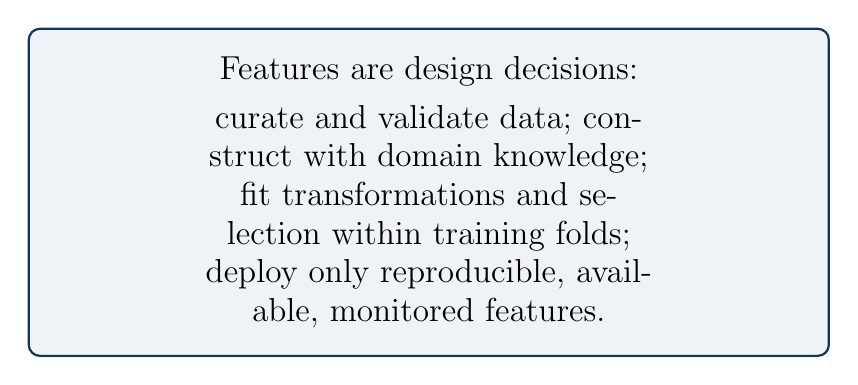
\begin{tikzpicture}
\node[fill=courseice, draw=courseblue, thick, rounded corners=4pt, inner sep=10pt, text width=0.78\textwidth, align=center, font=\large] {Features are design decisions:\\[0.3em] curate and validate data; construct with domain knowledge;\\ fit transformations and selection within training folds;\\ deploy only reproducible, available, monitored features.};
\end{tikzpicture}

\vfill
{\Large\bfseries\color{courseblue} Thank you for your attention.}

\vspace{0.4em}
{\small\color{coursegray} Next: Class 17 --- version control with Git.}
\vfill
\coursefooter
\end{frame}
\end{document}
